\documentclass{article}
\usepackage{amsmath}
\usepackage{graphicx}

\begin{document}
\title{PP1 Report}
\author{Logan Bontrager}
\maketitle

\section*{Task 1)}

In the first task, we test various estimate techniques under a bayesian unigram model. These include maximum likelihood, maximum a posterior, and the predictive distribution. The graph below shows the preplexity values of tested text data given a model trained on various training sizes.

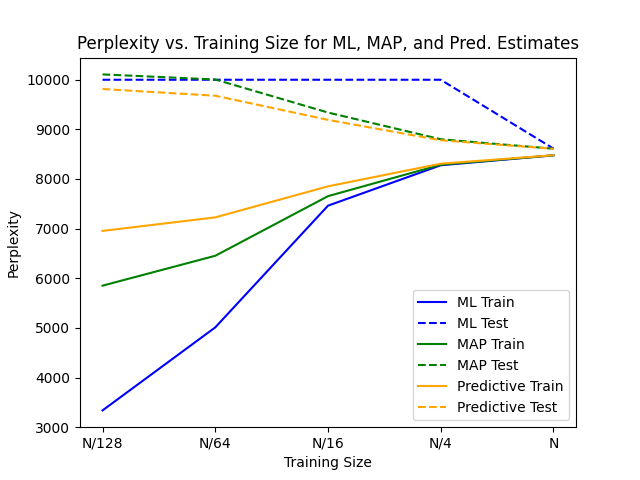
\includegraphics[width=\textwidth]{../output/task1.png}
Here, we see that as the training size increases the values for test and train perplexity converge. The testing values decrease because as we use more data, i.e., a larger training size, the true word frequencies or probability are better approximated. 
\\ \\
The maximum likelihood model performs rather poorly because of words in the testing set that don't appear in the training. Under the perplexity measure if a single word's probability is 0, the perplexity becomes infinity. This signifies poor model performance. The MAP and predictive methods fix this problem by assigning all words a base frequency of appearance through the use of a prior. This prior in conjunction with the data allows these methods to make better predictions which result in lower perplexity values as displayed in the graph. The predictive distribution takes this one step further and uses a weighted average of all models to best represent the distribution of words.
\\ \\
I think that the full training set will be moderately sensitive to changes in alpha. This is because alpha repesents a default appearance of a word in our underlying distribution. If the discrepancy between our prior and the true approximately average default appearance for words is large, than the model and test perplexity will be affected.


\section*{Task 2)}

Below is the graph of the bayesian unigram model under a predicitive distribution for a variety of alphas against both test perplexity and the log evidence.

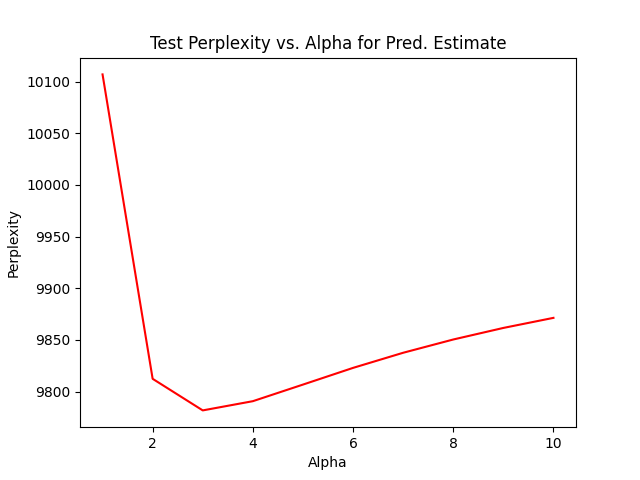
\includegraphics[width=\textwidth]{../output/task2pp.png}

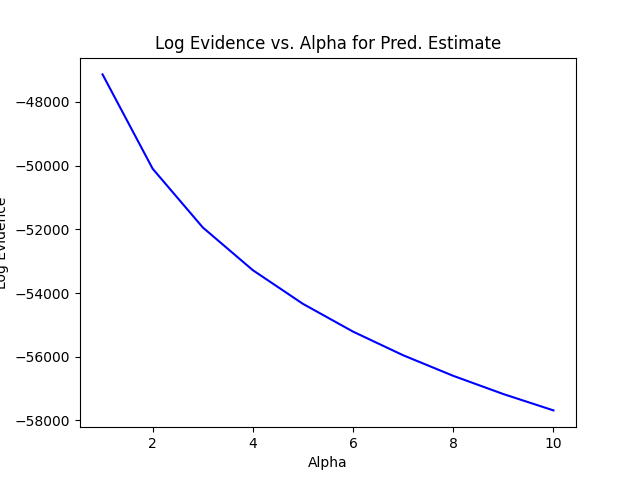
\includegraphics[width=\textwidth]{../output/task2evid.png}
Here, we see that the test perplexity is minimized when alpha is 3 and evidence is actually maximized when alpha is 0. Note that the evidence curve's derivative decreases slower as alpha increases. Thus under the assumption of minimizing complexity, evidence function maximization is not necessarily the best solution to finding a sufficient alpha for this dataset.


\section*{Task 3)}

In the third task, we try to test authorship of various pieces based on a predicitive model and text perplexity. For reference, the files 345 and 1188 under the pp1data folder are by B. Stoker and 84 is by M. Shelley. Initially, we trained the bayesian unigram model on 345. Then, we tested the perplexity of 1188 and 84 with this given model. An underlying assumption in this process is that an author has a consistent set of words he uses in his writing. Thus, two works or files by the same author will contain similar word frequencies. Therefore, in our tests the file 1188 should demonstrate a lower perplexity than 84 given the training than 84. 
\\ \\
After training and testing the model on the two files, we find that 1188 and 84 showed perplexities of 5542.54 and 7919.82 respectively. Thus, the model was effective in finding the work by the same author given the lower perplexity measure. 




\end{document}